\paragraph{\texttt{EquipmentModal}}  \mbox{}\\

This component displays a card for a given equipment, including its name, a brief description, and a link to see where
to buy it. Prior to \texttt{CourseCard}, the first table of is relatively straightforward.


\begin{center}
    \begin{tabularx}{\textwidth}{|X|X|X|X|}
        \hline
        \textbf{Prop} & Type & Required & Description \\
        \hline
        \texttt{equipment} & \texttt{Equipment} & yes & A yoga equipment \\
        \hline
    \end{tabularx}
\end{center}

And more precisely

\begin{center}
    \begin{tabularx}{\textwidth}{|X|X|X|}
        \hline
        \textbf{Prop.attribute} & Type & Description \\
        \hline
        \texttt{equipment.image} & \texttt{string | null} &  the path of the image associated with the yoga equipment stored in Supabase\\
        \hline
        \texttt{equipment.name} & \texttt{string} & the name of the yoga equipment\\
        \hline
        \texttt{equipment.description} & \texttt{string} & the publication date of the article\\
        \hline
        \texttt{equipment.purchase\_link} & \texttt{string} & a string that represents the URL of the partner's website\\
        \hline



    \end{tabularx}
\end{center}


\begin{figure}[H]
    \centering
    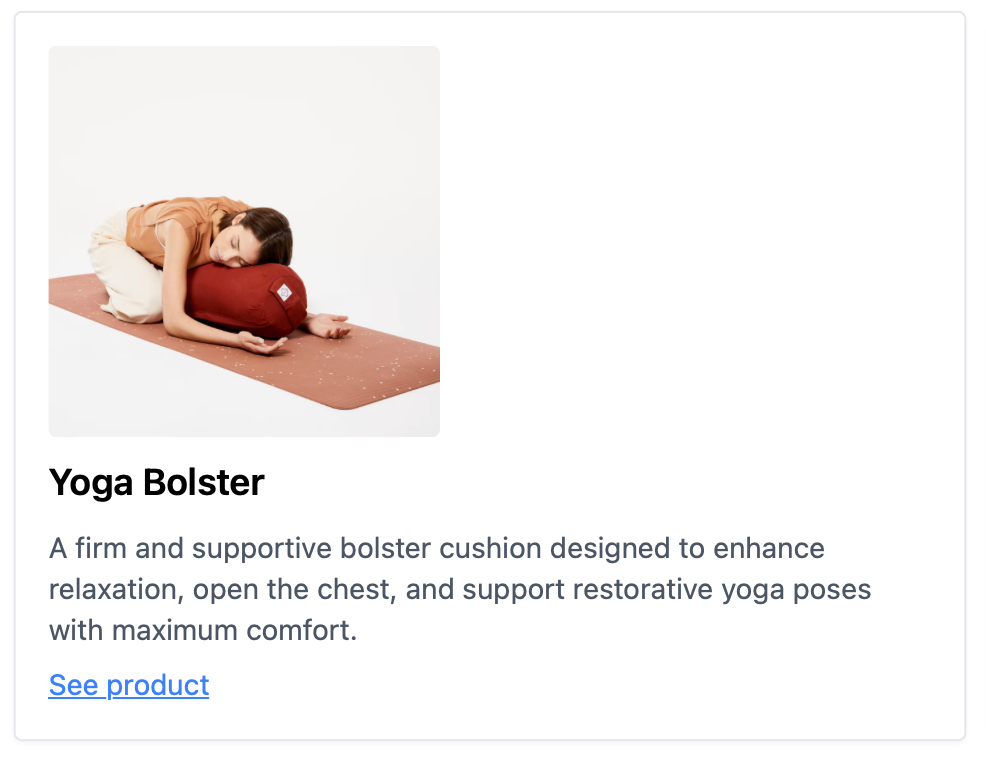
\includegraphics[width=0.2\textwidth]{asset/equipmentCard}
    \caption{\texttt{EquipmentCard}}
\end{figure}